\section{Motivation}

The study of spray jets is important for several technical applications: gas turbines, furnaces, automotive and rocket engines.  An extensive presentation of spray applications may be found in \cite{liu2000science}, but any equipment or transportation powered by the combustion of a liquid fuel has its design, efficiency and environmental impact challenged by the proper description of processes such as: liquid atomization, droplet transport, inter-phase transfers and vapor mixing with oxygen. Notwithstanding the expected complexity of all said, spray jets are often turbulent. 

Studying the spray jet by means of computer modeling alongside with experimentation is still a growing activity in industry, specially in what concerns brazilian activities. One notable difficulty is the requirement of expensive computational and laboratorial resources as well as capable professionals to operate them, and there is always doubt about how predictive/descriptive computations/experiments may be.

Undoubtful are, though, the benefits that society might receive from the evolution of technical applications: fuel flexibility, lower emission levels, higher work efficiency, safer operability.

\section{Objective}
This thesis has the following objectives:
\begin{itemize}
  \item Implement a low Mach number formulation to allow modeling of gas density variations due to high temperature gradients while neglecting fluid compressibility.
  \item Review some existent models for droplet-gas heat, mass and momentum transfers under the framework of RANS\footnote{RANS: Reynolds-averaged Navier-Stokes equations.} modeling for gas turbulence;
  \item Compare computed quantities to measurements reported in the literature such as droplet velocity and diameter, vapor and liquid mass flux, gas velocity and turbulence properties.
\end{itemize}

\section{The Spray Jet and the Lagrangian Point-Particle Method}

A spray jet is a particular case of a dispersed multiphase flow originated by the instabilization of a liquid jet emerging in a gaseous atmosphere.  The spray is composed by a continuous gaseous phase and a dispersed phase of liquid droplets. 

Differently from many multiphase flows where the description of phase interfaces is of great importance, in the dispersed regime it is the volume fraction of each phase the determinant factor of their interaction. The liquid volume fraction in spray jets may span from low or dilute ($\phi_{v,l} < 10^{-3}$) to high or dense ($\phi_{v,l} > 10^{-3}$).

In dilute sprays, the dynamics of liquid droplets is mainly governed by the gas turbulence. Modeling such sprays may be concentrated on modeling the gas effect on droplets and neglecting the droplet effect on the gas (one-way coupling) or taking both ways into account (two-way coupling). For dense sprays, however, the interaction between droplets (collision and coalescence) become important and must also be modeled (four-way coupling). A review on the computational approaches for different volume fractions is given in \cite{balachandar2010turbulent}. 

This work deals with a dilute spray ($\phi_{v,l} \approx 2.1 \times 10^{-5}$). A two-way coupling modeling was used for averaged flow properties and a one-way coupling was used for turbulence modeling; that is, no direct influence of droplets is present in the turbulence model equations and they are identical to those for a pure gaseous flow.

In the modeling formulation used in this work, the droplets were treated as point-particles with assigned properties and instead of tracking an interface, the problem is to track the droplet position in the domain. The Lagrangian point-particle nomenclature comes from the fact that droplet motion is described by ordinary differential equations written in a Lagrangian reference frame. This, coupled with the gaseous phase being modeled by partial differential equations in an Eulerian refence frame is what is called the Eulerian-Lagrangian description of the spray.

The interaction droplet-gas is done by computing source/sink terms to the gaseous equations and the correct droplet position must be known to correctly distribute the spray source terms in the gas flow. The more droplets are represented in the domain, smoother are the computed source terms.

\section{Low Mach Number Approximation}

In a subsonic flow at low Mach number, pressure variations affect the continuity equation much more by changing the velocity field than by changing the fluid density. If heat transfer is present, though, temperature variations may cause considerable variations in fluid density; and continuity, momentum and energy equations must be solved in a coupled manner. Solving the equations in the original compressible formulation adds unwanted difficulties to the numerical solver and requires extra care with the boundary conditions to avoid wave interferences in the solution \cite{poinsot2005theoretical}.

One possible approach is the Boussinesq simplification, which neglects density variations everywhere except in the buoyancy term in the momentum equation. This decouples the energy equation from both the momentum and continuity equations, but it is limited to low temperature differences of about $15K$ \cite{ferziger}.

In the case of a spray jet, temperature variations may be much higher and mass source terms are present due to droplet evaporation. Neglecting local changes in density may thus cause significant errors in the solution.

A possible way to overcome the limitations of the Boussinesq approximation and the complexity of the fully compressible formulation is the asymptotic approximation of zero Mach number for the Navier-Stokes equations. The simplified equations have been formally derived in \cite{majda} and are further discussed in \cite{muller1999low} and \cite{viozat1997implicit}.

For the spray jet studied in this thesis, the maximum Mach number is found in the nozzle exit and it is less than $0.1$.

\section{Droplet Evaporation}

A comprehensive text on droplet evaporation and heating is presented in \cite{sirignano}, where some covered topics are the case of a single and spherically symmetric droplet in a quiescent gas, the effect of gas convection around the droplet, the extra complexities of a multi-component liquid droplet, droplet behavior near critical conditions and the heating and evaporation of a group of droplets nearly located.

As previously mentioned, this thesis deals with a dilute spray and thus droplets are considered to heat and vaporize similarly to a single and isolated droplet. The effects of gas convection are taken into account using empirically established laws. The liquid phase has one single component (acetone) and the droplets are far from critical conditions.

Some more simplifications are made regarding the radial transport of heat inside the droplet. They will be discussed as the heating and the evaporation models are presented, in Chapter \ref{chap: equations}.

\section{Turbulence and Droplet Submodels}

\begin{figure}[h]
 \centering
\begin{tabular}{cc}
 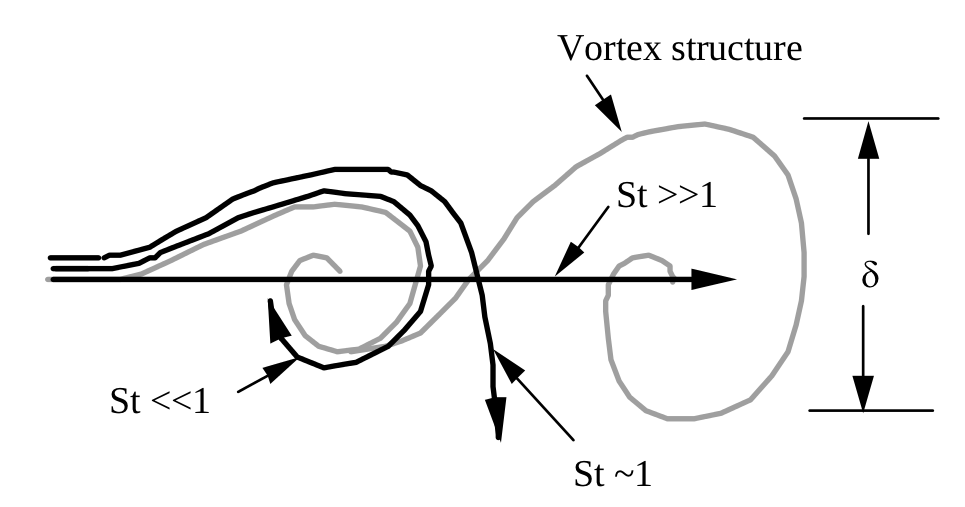
\includegraphics[width=0.75\textwidth]{./figuras/chap1/stokes.png}
\end{tabular}
 \caption{Effect of Stokes number on particle dispersion in large-scale turbulent structures, reproduced from \cite{crowe1988particle}.}
 \label{fig: intro_stokes}
\end{figure}

Apart all the implications concerning a multiphase flow, a spray jet is often turbulent, and the correct prediction of its evolution is dependent on how turbulence is modeled. It was said that the choice of the Lagrangian point-particle method to model the dispersed phase was based on the low liquid volume fraction. A second precaution is also very important when choosing the turbulence modeling for the gaseous flow and the dispersion modeling for the droplets. For spray jets where droplet Stokes number is very low ($St << 1$), see \cite{crowe1988particle} for the definition, the droplets are likely to completely follow oscillations in gas velocity and the interaction with turbulence is strong.

For such sprays, RANS modeling is likely to fail in predicting droplet motion and dispersion\footnote{Dispersion in the context of a spray is used in a similar sense to that in waves. It means that droplet velocity will be significantly dependent on its diameter as wave velocity would be dependent on frequency or wavenumber. } because the interaction with eddies will be restricted to some submodel.  The subject of turbulent dispersed multiphase flow is reviewed by \cite{balachandar2010turbulent} and the most important implications in droplet motion and evaporation are discussed in \cite{sirignano}.

In this work, the jet Reynolds number is not high ($Re=16,300$) and the Stokes number is $\left( St \in [1,100] \right)$ with an average of $10$. It is verified in Chapter \ref{chap: results} that the stochastic subgrid model used together with the traditional k-epsilon model was able to predict some dispersion in droplet velocities.

For the gas phase, it is a known fact that the k-epsilon model must have its coefficients tunned for improved accuracy in predicting the velocity field of a turbulent round jet. However, the exact modifications are not known \textit{a priori} and this work has used the usual coefficients. The consequences of this setup are discussed in Chapter \ref{chap: results}.

% \section{The OpenFOAM code}

% This thesis has made use of moderate computational resources and the open source software OpenFOAM\footnote{OpenFOAM is managed and distributed by the OpenFOAM Foundation and is freely available and open source, licensed under the GNU General Public Licence.}.

\section{Thesis Outline}

Chapter \ref{chap: equations} presents the governing equations for both the continuous and dispersed phases and the type of boundary conditions.
The continuous phase section starts with the fully compressible flow formulation, proceeds with the low Mach number approximation and then the averaging process of the turbulence modeling. The dispersed phase section describes the Lagrangian point-particle method and derives the models for momentum, heat and mass transfer between the droplets and the gas phase. 

Chapter \ref{chap: exp} briefly describes the experiment of \cite{chen}, which was used to evaluate the numerical results. It also presents the boundary conditions for the simulation obtained from the available experimental data.

Chapter \ref{chap: numerical} presents some aspects of the numerical solution such as the equation discretization schemes, the algorithms for solving linear systems and the mesh grid used for the domain discretization.

Chapter \ref{chap: results} presents the results and discussions. The first section presents the results for the properties of the gas phase turbulent jet: the spread rate and the self-similar profiles. The second section presents the results for droplet and gas velocities. The third section presents the mass fluxes of liquid and vapor and the droplet Sauter mean diameter.

Chapter \ref{chap: conclusion} summarizes the conclusions and suggestions for future work.

Appendix \ref{appendix 1} shows the derivation of the conservation equation of sensible enthalpy starting from the total energy equation.

Appendix \ref{appendix 2} show 2D Figures of droplet and gas properties.

Appendix \ref{appendix 3} briefly describes equation discretization and PISO algorithm.
